\def\retinaface{
    Mô hình RetinaFace \cite{deng2020retinaface} là một mô hình một pha giải quyết bài toán nhận diện khuôn mặt đạt kết quả tốt trên bộ dữ liệu WIDER FACE \cite{yang2016wider}.
    Mô hình RetinaFace được nhóm tác giả tích hợp nhiều mô hình và kỹ thuật khác nhau giúp nâng cao độ chính xác của mô hình.
    Ngoài ra, với việc sử dụng một mô hình backbone nhỏ hơn là Mobile-Net, mô hình RetinaFace có thể đạt tốc độ chạy trong thời gian thực trên CPU.

    \noindent
    \textbf{\textit{Kiến trúc mô hình RetinaFace}} \\
    Mô hình RetinaFace có kiến trúc dựa trên ý tưởng của RetinaNet \cite{lin2017focal} đã được thảo luận ở \textit{phần 2.3} của luận văn.
    RetinaFace cũng sử dụng kiến trúc backbone Feature Pyramids Network nhằm trích xuất đặc trưng của ảnh đầu vào với nhiều kích thước feature maps khác nhau.
    Tuy nhiên, thay vì sử dụng trực tiếp các feature maps này nhằm trả đầu ra là các bounding box chứa khuôn mặt, RetinaFace đưa các feature maps này qua các khối Context Module nhằm thu thập thêm các thông tin về background xung quanh trước khi đưa ra dự đoán về bounding box.
    
    \begin{figure}[H]
        \centering
        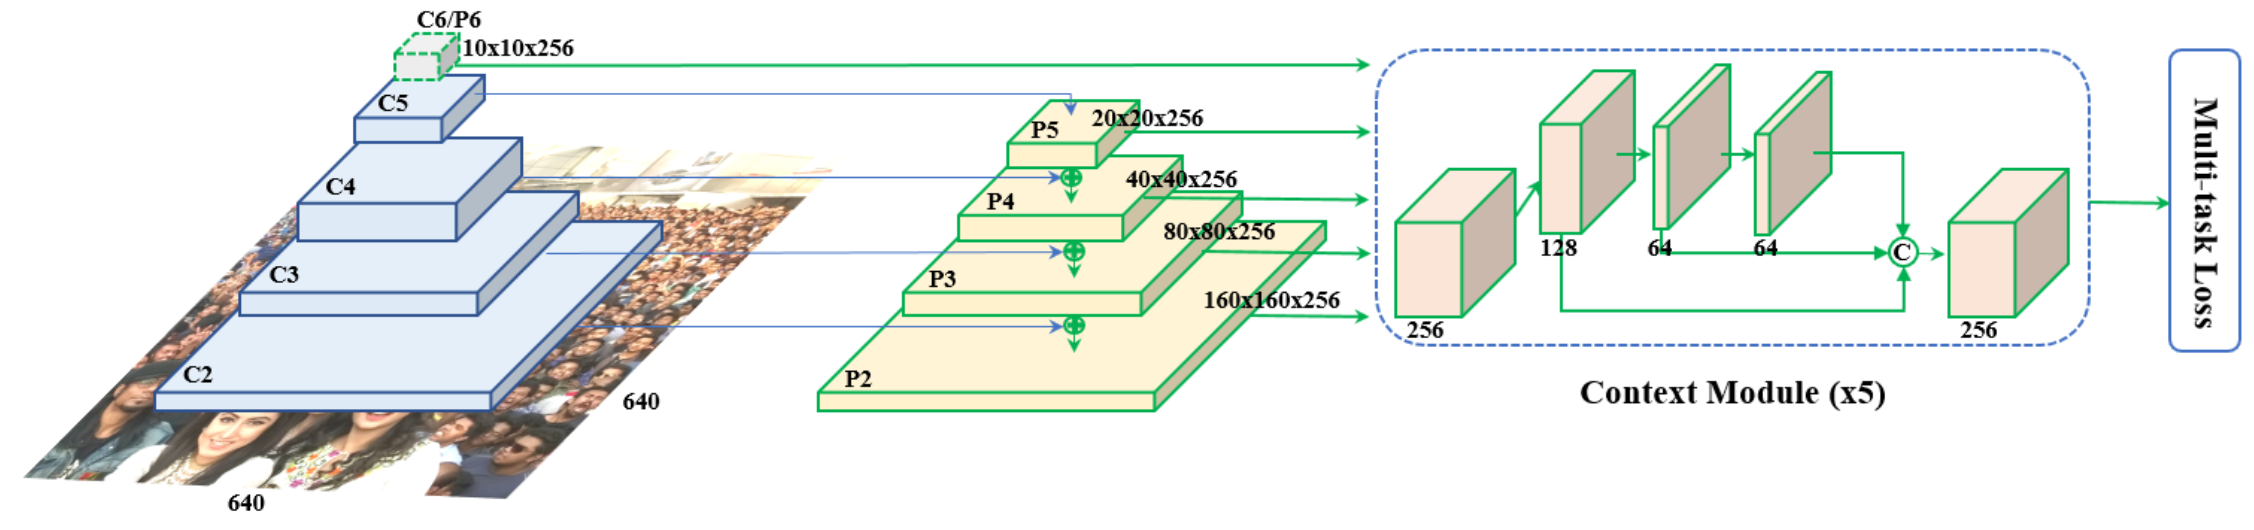
\includegraphics[width=10cm] {images/retinaface_architecture}
        \caption{Kiến trúc của mô hình RetinaFace. (Nguồn: \cite{deng2020retinaface})}
        \label{fig:retinaface_architecture}
    \end{figure}
    
    \noindent
    Ý tưởng sử dụng các khối Context Module tỏ ra khá hiệu quả khi áp dụng với bài toán nhận diện khuôn mặt.
    Đặc biệt trong việc định vị các mặt nhỏ, vì khi những thông tin về background xung quanh như thân người sẽ có vai trò quan trọng giúp mô hình học tốt hơn.
    Trong kiến trúc mô hình RetinaFace, bốn feature maps \textit{{${P}_{2}, {P}_{3}, {P}_{4}, {P}_{5}$}} của FPN và một feature maps \textit{{${C}_{6}$}} của backbone được đưa qua năm khối Context Module độc lập.
    Mỗi khối Context Module gồm ba khối Conv nối tiếp nhau, nhưng feature maps đầu ra của mỗi khối Conv đều được concat lại với nhau để tạo ra feature maps cuối cùng của cả khối Context Module.
    Trong thực tế, nhằm đạt kết quả tốt nhất trên bộ dữ liệu WIDER FACE, mô hình RetinaFace sử dụng kỹ thuật \textit{deformable convolution network} (gọi tắt là DCN) thay thế cho các lớp Conv truyền thống.

    \noindent
    \textbf{\textit{Hệ thống các hàm loss của mô hình RetinaFace}} \\
    Việc nhóm tác giả đã bổ sung thêm landmarks của các khuôn mặt trên bộ WIDER FACE (đã được nhắc đến tại \textit{phần 4.1} của luận văn) đã giúp mô hình RetinaFace có thể xây dựng và tối ưu hàm loss multi-task.

    \begin{figure}[H]
        \centering
        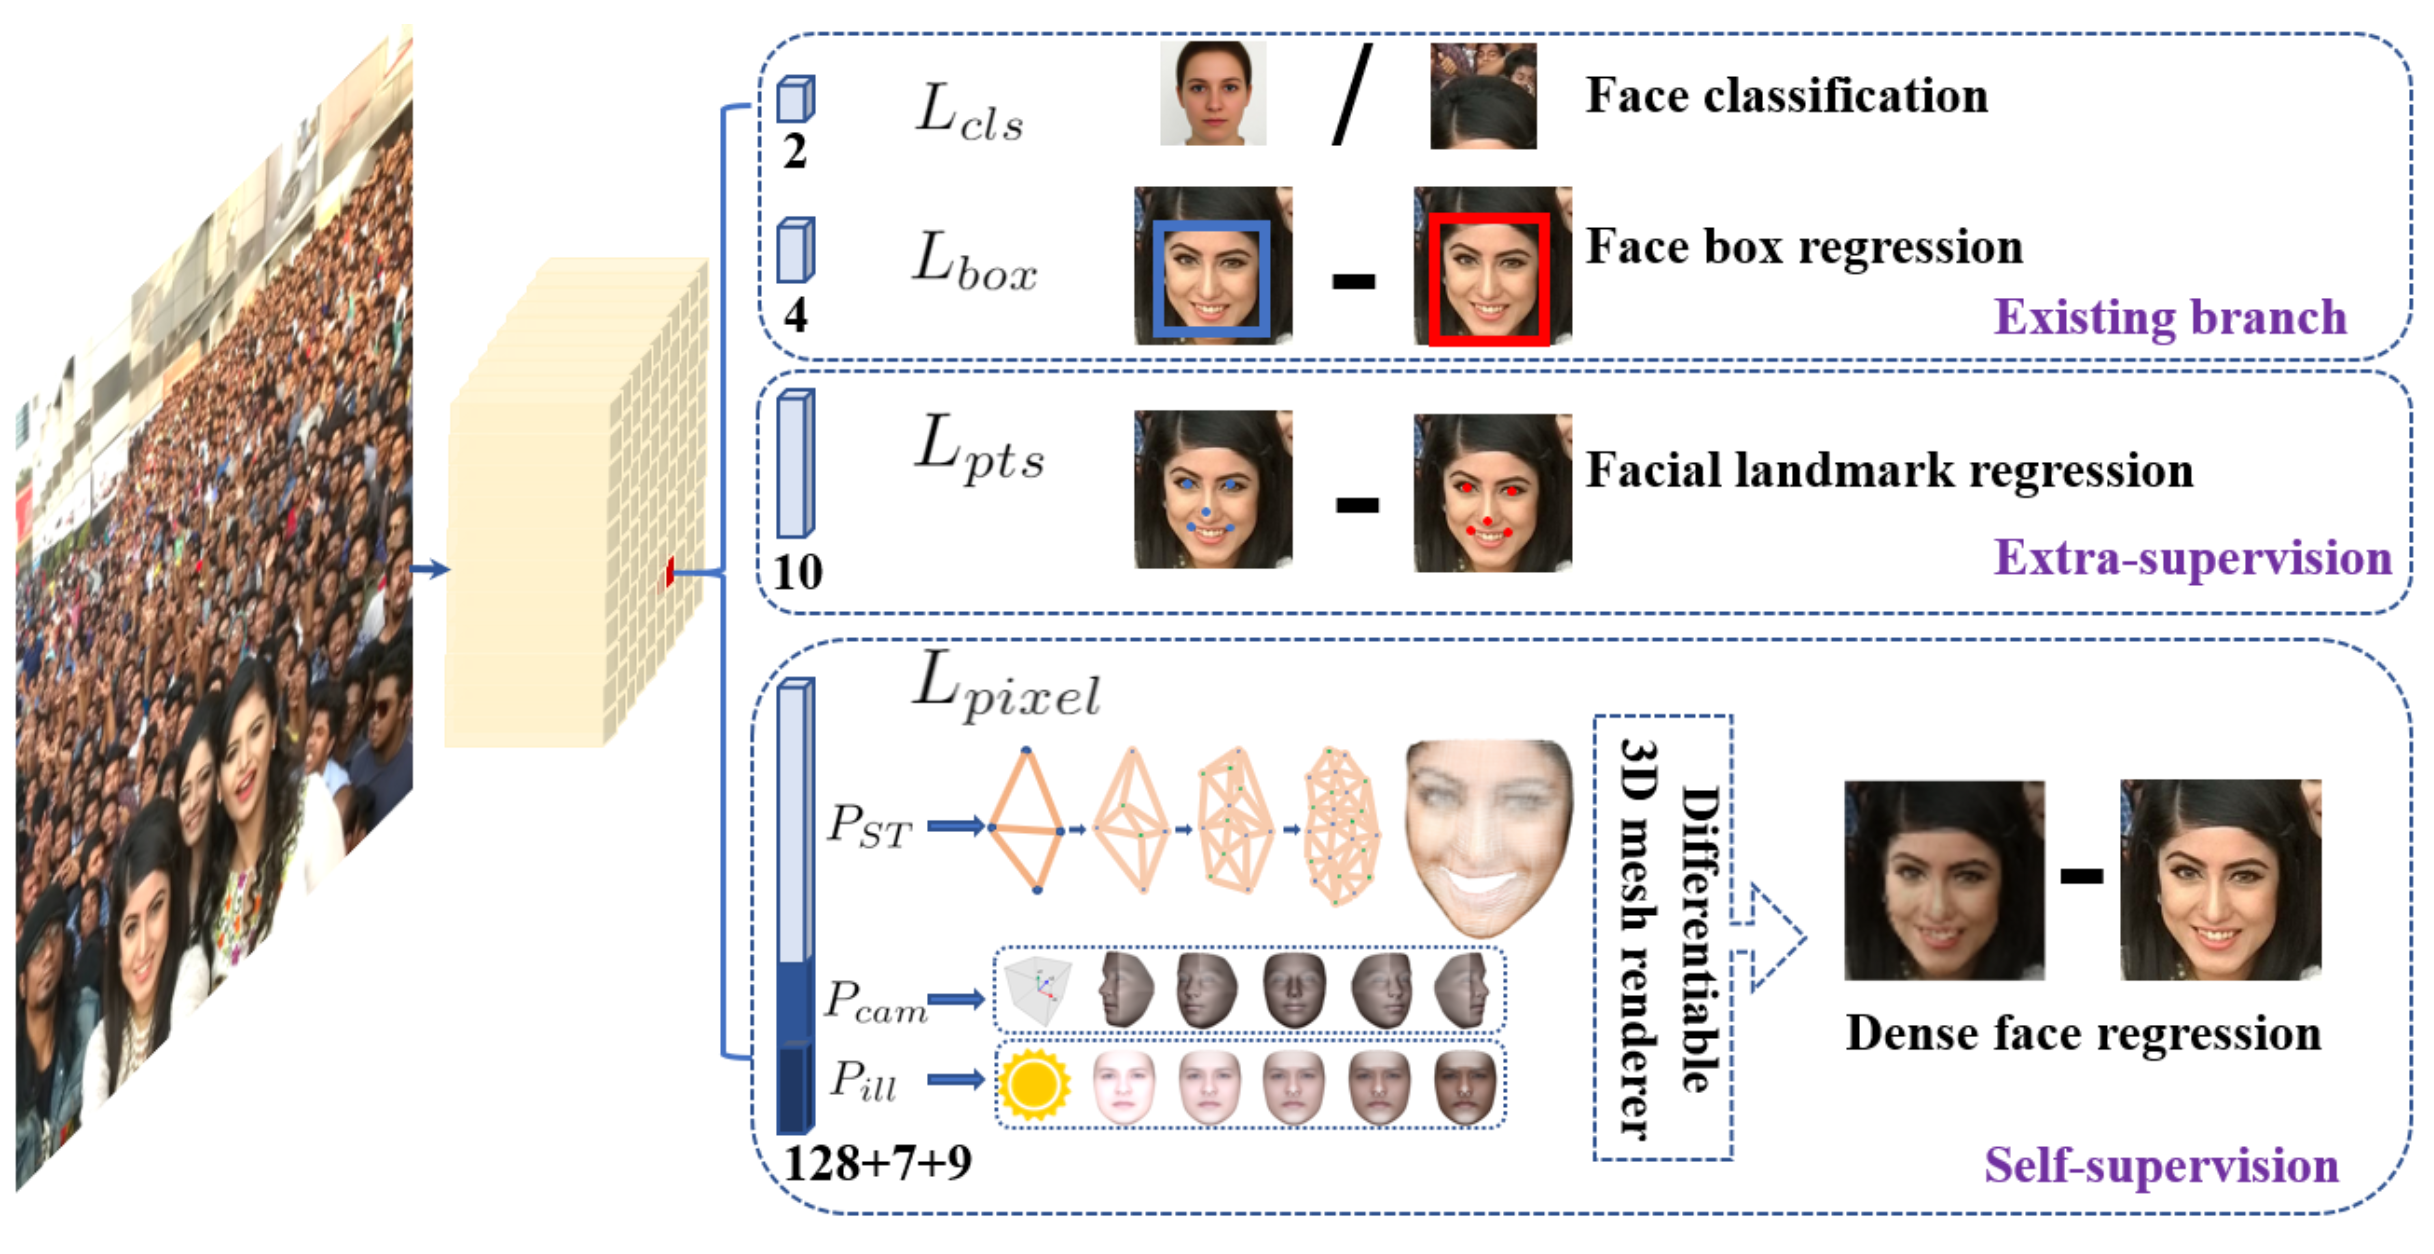
\includegraphics[width=10cm] {images/retinaface_loss_funcs}
        \caption{Ý tưởng hàm loss multi-task của mô hình RetinaFace. (Nguồn: \cite{deng2020retinaface})}
        \label{fig:retinaface_loss_funcs}
    \end{figure}

    Cụ thể hơn, trong quá trình train mô hình, với mỗi anchor, mô hình RetinaFace tối ưu hàm loss multi-task dưới đây:

    \begin{equation}
        \begin{split}
        L  & =  L_{cls}(p_i, p^{*}_i) + \lambda_1 p^{*}_i L_{box}(t_i, t^{*}_i) + \lambda_2 p^{*}_i L_{pts} (l_i, l^{*}_i) + \lambda_3 p^{*}_i L_{pixel}.\\
        \end{split}
        \label{eq:retinaface_loss}
    \end{equation}

    \noindent
    trong đó: \\
    - Các trọng số $\lambda_1, \lambda_2, \lambda_3$ được nhóm tác giả cấu hình mặc định là 0.25, 0.1 và 0.01. \\
    - Hàm loss phân lớp mặt: \\
    $L_{cls}(p_i, p^{*}_i)$ với $p_i$ là xác suất mà mô hình dự đoán một anchor có chứa là khuôn mặt hay không.
    Ta có $p^{*}_i = 1$ nếu anchor đó chứa khuôn mặt còn $p^{*}_i = 0$ nếu anchor đó không chứa khuôn là mặt. \\
    - Hàm loss hồi quy định vị vị trí của bbox: \\
    $L_{box}(t_i, t^{*}_i)$ với $t_i=\{t_x, t_y, t_w, t_h\}_i$ và $t^{*}_i=\{t^{*}_x, t^{*}_y, t^{*}_w, t^{*}_h\}_i$ lần lượt là bộ bốn tham số đại diện cho toạ độ của anchor mà mô hình dự đoán là mặt và bbox ground-truth từ bộ dữ liệu.
    (x là toạ độ x của điểm góc trái trên, y là toạ độ y của điểm góc trái trên, w là chiều rộng của bbox và h là chiều cao của bbox). \\
    - Hàm loss hồi quy định vị vị trí của landmarks: \\
    $L_{pts} (l_i, l^{*}_i)$ với $l_i=\{l_{x_1}, l_{y_1}, \dots , l_{x_5}, l_{y_5}\}_i$ và $l^{*}_i=\{l^{*}_{x_1}, l^{*}_{y_1}, \dots , l^{*}_{x_5}, l^{*}_{y_5}\}_i$ lần lượt là bộ mười tham số đại diện cho toạ độ của năm landmarks mà mô hình dự đoán ứng với mỗi bounding box dự đoán và năm ground-truth landmarks của mỗi groundtruth bounding box từ bộ dữ liệu. \\
    - Hàm loss hồi quy từng pixel của khuôn mặt: $L_{pixel}$ giúp bổ sung thêm thông tin và giúp loại bớt các trường hợp dự đoán nhầm background là khuôn mặt của mô hình. \\
    Hàm loss $L_{pixel}$ của mô hình RetinaFace là một hàm loss self-supervised learning.
    Cụ thể, RetinaFace sử dụng nghiên cứu \cite{zhou2019dense} dựa trên Graph Convolution Network để biến đối khuôn mặt từ bounding box trên ảnh sang dạng 3D, sau đó sử dụng mô hình \cite{genova2018unsupervised} để biến đổi ngược từ khuôn mặt dạng 3D trở về dạng 2D như trên ảnh thông thường.

    \begin{equation}
        L_{pixel}  = \frac{1}{W*H} \sum_{i}^{W} \sum_{j}^{H}  \|\mathcal{R}(\mathcal{D}_{P_{ST}},P_{cam},P_{ill})_{i,j} - I_{i,j}^*\|_1,\\
        \label{fig:retinaface_loss_pixel}
    \end{equation}

    \noindent
    trong đó: \\
    - $\mathcal{D}_{P_{ST}}$ là khuôn mặt sau khi biến đổi từ bounding box sang dạng 3D theo nghiên cứu \cite{zhou2019dense}. \\
    - $\mathcal{R}$ là mô hình biến đổi từ khuôn mặt dạng 3D trở về dạng 2D như trên ảnh thông thường theo nghiên cứu \cite{genova2018unsupervised}. \\
    - $P_{cam}, P_{ill}$ là các tham số của mô hình \cite{genova2018unsupervised}. \\
    - $W$ và $H$ lần lượt là chiều rộng và chiều dài của bounding box $I^*$.

    \noindent
    \textbf{\textit{Kết quả của mô hình RetinaFace}} \\
    Nhóm tác giả thực hiện thí nghiệm đánh giá mức độ đóng góp của các kỹ thuật trong mô hình RetinaFace. \\
    - FPN+Context: mô hình RetinaFace chỉ sử dụng kiến trúc FPN kết hợp các khối Context Module \cite{najibi2017ssh} với lớp Conv truyền thống. \\
    - +DCN: mô hình RetinaFace chỉ sử dụng kiến trúc FPN kết hợp các khối Context Module \cite{najibi2017ssh} với deformable convolution network \cite{dai2017deformable}. \\
    - +$L_{pts}$: mô hình RetinaFace chỉ sử dụng kiến trúc FPN kết hợp các khối Context Module \cite{najibi2017ssh} với deformable convolution network \cite{dai2017deformable} bổ sung thêm hàm loss về năm điểm landmarks. \\
    - +$L_{pixel}$: mô hình RetinaFace chỉ sử dụng kiến trúc FPN kết hợp các khối Context Module \cite{najibi2017ssh} với deformable convolution network \cite{dai2017deformable} bổ sung thêm hàm loss về self-supervised learning. \\
    - +$L_{pts}$+$L_{pixel}$: mô hình RetinaFace chỉ sử dụng kiến trúc FPN kết hợp các khối Context Module \cite{najibi2017ssh} với deformable convolution network \cite{dai2017deformable} bổ sung thêm hàm loss về năm điểm landmarks và hàm loss về self-supervised learning. \\

    \begin{figure}[H]
        \centering
        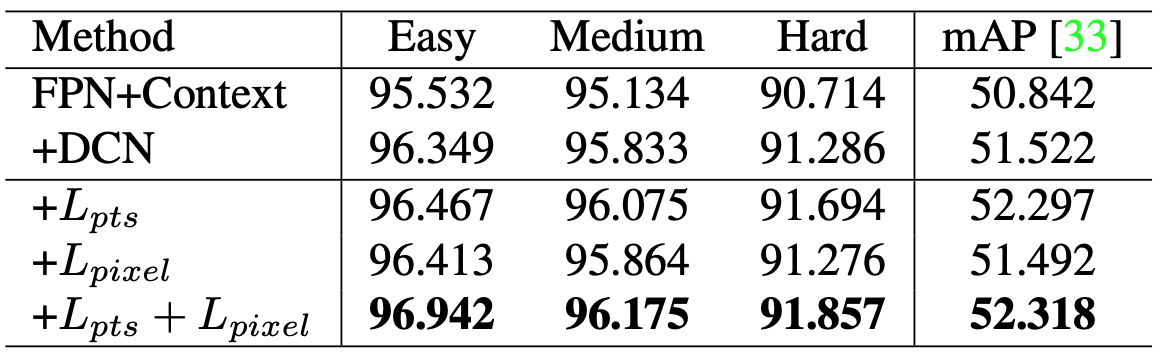
\includegraphics[width=10cm] {images/retinaface_results_1}
        \caption{So sánh kết quả việc sử dụng một số kỹ thuật trong mô hình RetinaFace. (Nguồn: \cite{deng2020retinaface})}
        \label{fig:retinaface_results_1}
    \end{figure}

    \noindent
    Cấu hình RetinaFace sử dụng tất cả các kỹ thuật trên cho kết quả tốt nhất trên cả ba bộ WIDER FACE val dễ, trung bình và khó.

    \noindent
    Việc mô hình RetinaFace cho kết quả tốt trên bài toán nhận diện khuôn mặt giúp cải thiện kết quả của mô hình ArcFace trên bài toán face recognition trên các bộ dữ liệu khác nhau. \\
    - MTCNN+ArcFace: là cấu hình sử dụng mô hình MTCNN \cite{zhang2016joint} cho bài toán nhận diện khuôn mặt và mô hình ArcFace \cite{deng2019arcface} cho bài toán face recognition. \\
    - RetinaFace+ArcFace: là cấu hình sử dụng mô hình RetinaFace cho bài toán nhận diện khuôn mặt và mô hình ArcFace \cite{deng2019arcface} cho bài toán face recognition.

    \begin{figure}[H]
        \centering
        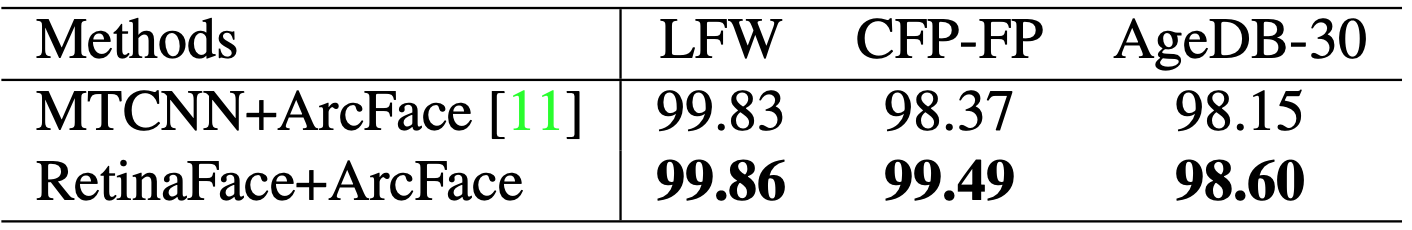
\includegraphics[width=10cm] {images/retinaface_results_2}
        \caption{Kết quả tốt của mô hình RetinaFace trên bài toán nhận diện khuôn mặt giúp cải thiện kết quả trên cả bài toán face recognition. (Nguồn: \cite{deng2020retinaface})}
        \label{fig:retinaface_results_2}
    \end{figure}

    \noindent
    Ở thời điểm ra mắt, mô hình RetinaFace cho kết quả tốt nhất trên tất cả các bộ dữ liệu con của bộ WIDER FACE, bao gồm: \\
    - Với bộ val dễ đạt: 96.9\% \\
    - Với bộ val trung bình đạt: 96.1\% \\
    - Với bộ val khó đạt: 91.8\% \\
    - Với bộ test dễ đạt: 96.3\% \\
    - Với bộ test trung bình đạt: 95.6\% \\
    - Với bộ test khó đạt: 91.4\%

    \begin{figure}[H]
        \centering
        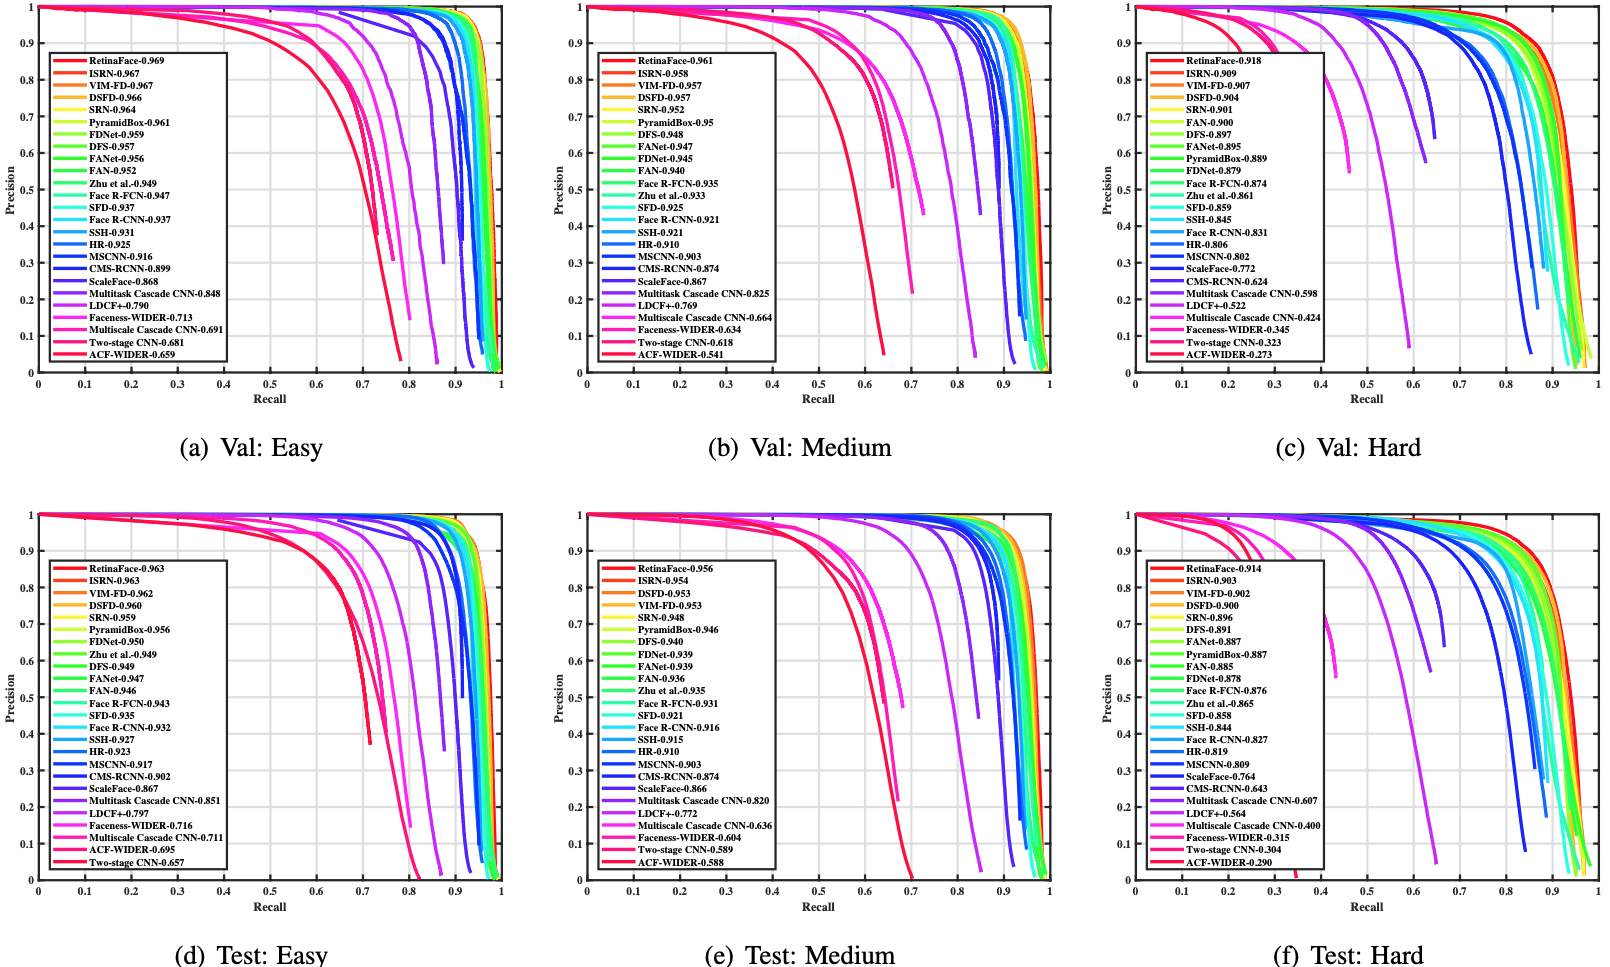
\includegraphics[width=10cm] {images/retinaface_results_3}
        \caption{Kết quả của về Precision - Recall của mô hình RetinaFace trên các bộ dữ liệu con của WIDER FACE. (Nguồn: \cite{deng2020retinaface})}
        \label{fig:retinaface_results_3}
    \end{figure}

    \noindent
    \textbf{\textit{Vấn đề tồn đọng của mô hình RetinaFace}} \\
    Mô hình RetinaFace đã giải quyết bài toán nhận diện khuôn mặt với bộ dữ liệu WIDER FACE rất tốt, đạt độ chính xác cao.
    Tuy nhiên, khi xử lý với ảnh có kích thước lớn, mô hình RetinaFace muốn giữ được kết quả tốt cần mất thời gian chạy khá lâu.
    Điều này khiến cho mô hình RetinaFace thường chỉ nằm ở mức độ nghiên cứu và khó có thể được sử dụng trong các ứng dụng thực tế.
}